% =====================================================================
%  Capítulo 18. Cópulas
% =====================================================================
\chapter[Cópulas]{Cópulas: dependencia más allá de la correlación}\label{cap:copulas}

\section*{Objetivos de aprendizaje}
Al terminar este capítulo, el lector podrá:
\begin{enumerate}[label=\arabic*.,leftmargin=*]
  \item Separar una distribución conjunta en sus márgenes y su cópula (teorema de Sklar) y entender por qué la
        cópula es la parte que mide la dependencia.
  \item Calcular las medidas de dependencia que solo dependen de la cópula (tau de Kendall, rho de Spearman,
        dependencia en las colas) y derivarlas para las familias gaussiana, $t$, Clayton y Gumbel.
  \item Estimar cópulas por máxima verosimilitud canónica con pseudo-observaciones y compararlas.
  \item Simular de una cópula y usarla para medir el riesgo de una cartera.
\end{enumerate}

\section*{Motivación}
La correlación de Pearson resume la dependencia entre dos rendimientos con un número, pero ese número tiene tres
limitaciones. Solo mide asociación lineal; cambia si se transforma una variable (la correlación de dos precios no es la
de sus logaritmos); y no dice nada sobre lo que más le importa a un gestor de riesgos: si los activos caen \emph{juntos}
en los días malos. Dos pares de activos pueden tener la misma correlación y comportamientos muy distintos en las colas.
Una cópula describe la estructura completa de la dependencia, separada de las distribuciones de cada activo. Desde
que Embrechts, McNeil y Straumann (2002) mostraron los peligros de la correlación, las cópulas son una herramienta
estándar del riesgo de mercado y de crédito, y también una advertencia: el uso de la cópula gaussiana para valorar
obligaciones de deuda garantizada contribuyó a subestimar el riesgo antes de la crisis de 2008 (MacKenzie y Spears, 2014).

\paragraph{Datos del capítulo.} Rendimientos logarítmicos diarios (en porcentaje) del S\&P 500 y del índice compuesto
Nasdaq, del 5 de enero de 1999 al 31 de diciembre de 2018 ($n=5\,030$), de Yahoo Finance.

% ---------------------------------------------------------------------
\section{Cópulas y el teorema de Sklar}
% ---------------------------------------------------------------------

\begin{definicion}[Cópula]
Una cópula bivariada es la función de distribución conjunta $C(u,v)=\Pr(U\le u,V\le v)$ de un vector $(U,V)$ cuyas dos
márgenes son uniformes en $[0,1]$.
\end{definicion}

El resultado que conecta las cópulas con cualquier distribución es la \emph{transformación integral de probabilidad}.

\begin{proposicion}[Transformación integral de probabilidad]\label{prop:tip}
Si $X$ tiene función de distribución continua y estrictamente creciente $F$, entonces $U=F(X)$ es uniforme en $[0,1]$.
\end{proposicion}

\begin{proof}
Para $u\in(0,1)$, como $F$ es estrictamente creciente, $F(X)\le u$ equivale a $X\le F^{-1}(u)$:
\begin{align*}
  \Pr(U\le u) &= \Pr\bigl(F(X)\le u\bigr)\\
              &= \Pr\bigl(X\le F^{-1}(u)\bigr)\\
              &= F\bigl(F^{-1}(u)\bigr)\\
              &= u .
\end{align*}
\end{proof}

\begin{proposicion}[Teorema de Sklar, caso continuo]\label{prop:sklar}
Sea $H$ la distribución conjunta de $(X,Y)$ con márgenes continuas y estrictamente crecientes $F$ y $G$. Existe una única
cópula $C$ tal que
\[
  H(x,y)=C\bigl(F(x),G(y)\bigr)\quad\text{para todo }(x,y),
\]
y es $C(u,v)=H\bigl(F^{-1}(u),G^{-1}(v)\bigr)$. Recíprocamente, para cualquier cópula $C$ y márgenes $F$, $G$, la
función $C(F(x),G(y))$ es una distribución conjunta con esas márgenes.
\end{proposicion}

\begin{proof}
Sean $U=F(X)$ y $V=G(Y)$, uniformes por la Proposición~\ref{prop:tip}, y $C$ su distribución conjunta, que es una cópula.
Entonces
\begin{align*}
  H(x,y) &= \Pr(X\le x,\ Y\le y)\\
         &= \Pr\bigl(F(X)\le F(x),\ G(Y)\le G(y)\bigr)\\
         &= \Pr\bigl(U\le F(x),\ V\le G(y)\bigr)\\
         &= C\bigl(F(x),G(y)\bigr),
\end{align*}
donde el segundo paso usa que $F$ y $G$ son estrictamente crecientes. Evaluando en $x=F^{-1}(u)$, $y=G^{-1}(v)$ se obtiene la
fórmula de $C$, que la determina por completo: es única. Para el recíproco, si $(U,V)\sim C$, el vector
$(F^{-1}(U),G^{-1}(V))$ tiene márgenes $F$ y $G$ (por el mismo argumento al revés) y distribución conjunta $C(F(x),G(y))$.
\end{proof}

Sklar dice que toda distribución conjunta es \emph{márgenes más cópula}, y que ambas partes pueden elegirse por separado.
Esto permite modelar cada rendimiento con la distribución que mejor le ajuste (una $t$, un GARCH, la empírica) y la
dependencia con otra herramienta.

\begin{proposicion}[Invariancia]\label{prop:invariancia}
Si $g_1$ y $g_2$ son estrictamente crecientes, $(g_1(X),g_2(Y))$ tiene la misma cópula que $(X,Y)$.
\end{proposicion}

\begin{proof}
La distribución de $X'=g_1(X)$ es $F'(x')=F(g_1^{-1}(x'))$, de modo que $F'(X')=F(g_1^{-1}(g_1(X)))=F(X)=U$; igual para $Y'$.
Por tanto,
\begin{align*}
  C'(u,v) &= \Pr\bigl(F'(X')\le u,\ G'(Y')\le v\bigr)\\
          &= \Pr\bigl(F(X)\le u,\ G(Y)\le v\bigr)\\
          &= C(u,v).
\end{align*}
\end{proof}

La correlación de Pearson \emph{no} es invariante: si $X\sim N(0,1)$ e $Y=e^X$, la cópula es la de la dependencia perfecta,
pero $\operatorname{Corr}(X,Y)=1/\sqrt{e-1}=0{,}763$ (Ejercicio propuesto 18.3). Las medidas que solo dependen de la cópula sí lo son.

\begin{proposicion}[Cotas de Fréchet-Hoeffding]\label{prop:frechet}
Toda cópula cumple $W(u,v)=\max(u+v-1,0)\le C(u,v)\le\min(u,v)=M(u,v)$.
\end{proposicion}

\begin{proof}
Cota superior: el suceso $\{U\le u,V\le v\}$ está contenido en $\{U\le u\}$ y en $\{V\le v\}$:
\begin{align*}
  C(u,v) &\le \Pr(U\le u)=u,\\
  C(u,v) &\le \Pr(V\le v)=v,\\
  C(u,v) &\le \min(u,v).
\end{align*}
Cota inferior: por la desigualdad de Bonferroni, $\Pr(A\cap B)\ge\Pr(A)+\Pr(B)-1$:
\begin{align*}
  C(u,v) &= \Pr(\{U\le u\}\cap\{V\le v\})\\
         &\ge u+v-1,
\end{align*}
y como una probabilidad no es negativa, $C(u,v)\ge\max(u+v-1,0)$.
\end{proof}

$M$ es la cópula de la \emph{comonotonía} ($V=U$: los activos se mueven siempre en el mismo sentido), $W$ la de la
\emph{contramonotonía} ($V=1-U$) y $\Pi(u,v)=uv$ la de la independencia (Figura~\ref{fig:frechet}).

\begin{figure}[ht]
\centering
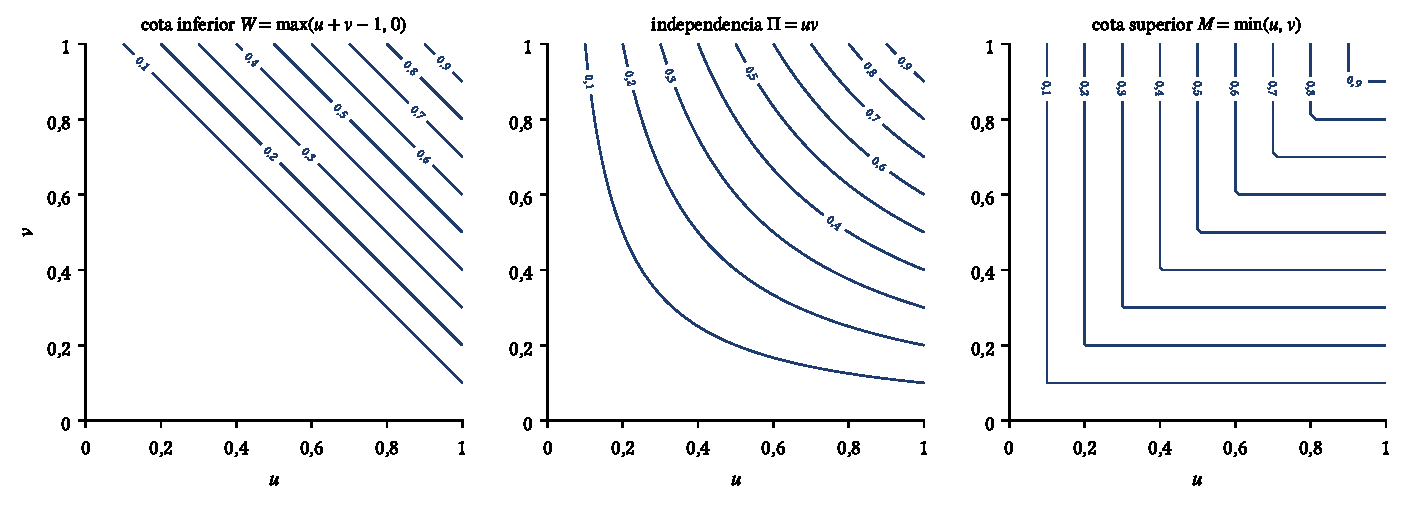
\includegraphics[width=\linewidth]{graficos/cap18_fig_frechet.pdf}
\caption{Curvas de nivel de las cotas de Fréchet-Hoeffding y de la cópula de independencia. Toda cópula está entre la
primera y la tercera.}
\label{fig:frechet}
\end{figure}

\paragraph{Densidad y verosimilitud.} Si $C$ tiene densidad $c(u,v)=\partial^2C/\partial u\,\partial v$, derivando
$H(x,y)=C(F(x),G(y))$ por la regla de la cadena,
\[
  h(x,y)=c\bigl(F(x),G(y)\bigr)\,f(x)\,g(y),\qquad
  \ln h=\ln c\bigl(F(x),G(y)\bigr)+\ln f(x)+\ln g(y).
\]
La log-verosimilitud se separa en una parte de la cópula y otra de cada margen.

% ---------------------------------------------------------------------
\section{Familias de cópulas}
% ---------------------------------------------------------------------

\paragraph{Cópulas elípticas.} La cópula gaussiana con correlación $\rho$ es la de una normal bivariada:
$C(u,v)=\Phi_2\bigl(\Phi^{-1}(u),\Phi^{-1}(v);\rho\bigr)$. La cópula $t$ es la de una $t$ bivariada con $\nu$ grados de
libertad.

\begin{proposicion}[Densidad de la cópula gaussiana]\label{prop:densgauss}
Con $x=\Phi^{-1}(u)$ e $y=\Phi^{-1}(v)$,
\[
  c(u,v)=\frac{1}{\sqrt{1-\rho^2}}\exp\Bigl(-\frac{\rho^2(x^2+y^2)-2\rho xy}{2(1-\rho^2)}\Bigr).
\]
\end{proposicion}

\begin{proof}
Por la descomposición de la densidad con márgenes normales,
\[
  c(u,v)=\frac{\phi_2(x,y;\rho)}{\phi(x)\,\phi(y)}:
\]
\begin{align*}
  c(u,v) &= \frac{\frac{1}{2\pi\sqrt{1-\rho^2}}\exp\bigl(-\frac{x^2-2\rho xy+y^2}{2(1-\rho^2)}\bigr)}{\frac{1}{2\pi}\exp\bigl(-\frac{x^2+y^2}{2}\bigr)}\\
         &= \frac{1}{\sqrt{1-\rho^2}}\exp\Bigl(-\frac{x^2-2\rho xy+y^2}{2(1-\rho^2)}+\frac{(1-\rho^2)(x^2+y^2)}{2(1-\rho^2)}\Bigr)\\
         &= \frac{1}{\sqrt{1-\rho^2}}\exp\Bigl(-\frac{\rho^2(x^2+y^2)-2\rho xy}{2(1-\rho^2)}\Bigr).
\end{align*}
\end{proof}

\paragraph{Cópulas arquimedianas.} Se construyen con un \emph{generador} $\varphi$ continuo, decreciente y convexo con
$\varphi(1)=0$: $C(u,v)=\varphi^{-1}\bigl(\varphi(u)+\varphi(v)\bigr)$. Las dos más usadas en finanzas son
\begin{itemize}[leftmargin=*]
  \item \textbf{Clayton}: $\varphi(t)=(t^{-\theta}-1)/\theta$, $\theta>0$, de modo que $C(u,v)=(u^{-\theta}+v^{-\theta}-1)^{-1/\theta}$;
  \item \textbf{Gumbel}: $\varphi(t)=(-\ln t)^\theta$, $\theta\ge1$, de modo que
        $C(u,v)=\exp\bigl\{-[(-\ln u)^\theta+(-\ln v)^\theta]^{1/\theta}\bigr\}$.
\end{itemize}

\paragraph{Medidas de concordancia.} El tau de Kendall es la probabilidad de que dos pares independientes sean
concordantes menos la de que sean discordantes; el rho de Spearman es la correlación de Pearson de $(U,V)$. Ambas
dependen solo de la cópula: $\tau=4\E[C(U,V)]-1$ y $\rho_S=12\iint C(u,v)\,du\,dv-3$. Para las cópulas elípticas,
$\tau=\frac2\pi\arcsin\rho$ (Lindskog, McNeil y Schmock, 2003), y para las arquimedianas, $\tau=1+4\int_0^1\varphi(t)/\varphi'(t)\,dt$
(Genest y MacKay, 1986).

\begin{proposicion}[Tau de Kendall de Clayton y de Gumbel]\label{prop:taukendall}
Para Clayton, $\tau=\theta/(\theta+2)$; para Gumbel, $\tau=1-1/\theta$.
\end{proposicion}

\begin{proof}
Clayton: $\varphi'(t)=-t^{-\theta-1}$, de modo que
\begin{align*}
  \frac{\varphi(t)}{\varphi'(t)} &= -\frac{(t^{-\theta}-1)\,t^{\theta+1}}{\theta}\\
                                 &= -\frac{t-t^{\theta+1}}{\theta},\\
  \int_0^1\frac{\varphi(t)}{\varphi'(t)}\,dt &= -\frac1\theta\Bigl(\frac12-\frac1{\theta+2}\Bigr)\\
                                             &= -\frac1\theta\cdot\frac{\theta}{2(\theta+2)}\\
                                             &= -\frac{1}{2(\theta+2)},\\
  \tau &= 1-\frac{4}{2(\theta+2)}\\
       &= \frac{\theta}{\theta+2}.
\end{align*}
Gumbel: $\varphi'(t)=-\theta(-\ln t)^{\theta-1}/t$, de modo que
\begin{align*}
  \frac{\varphi(t)}{\varphi'(t)} &= -\frac{t\,(-\ln t)^\theta}{\theta(-\ln t)^{\theta-1}}\\
                                 &= \frac{t\ln t}{\theta},\\
  \int_0^1t\ln t\,dt &= \Bigl[\frac{t^2\ln t}{2}\Bigr]_0^1-\int_0^1\frac t2\,dt\\
                     &= 0-\frac14,\\
  \tau &= 1+\frac4\theta\Bigl(-\frac14\Bigr)\\
       &= 1-\frac1\theta .
\end{align*}
\end{proof}

\paragraph{Dependencia en las colas.} Los coeficientes de dependencia en la cola inferior y superior son
\[
  \lambda_L=\lim_{q\to0^+}\Pr(V\le q\mid U\le q)=\lim_{q\to0^+}\frac{C(q,q)}{q},\qquad
  \lambda_U=\lim_{q\to1^-}\Pr(V>q\mid U>q).
\]
Miden la probabilidad de que un activo tenga un día extremo dado que el otro lo tuvo.

\begin{proposicion}[Dependencia en las colas de Clayton y de Gumbel]\label{prop:colas}
Clayton: $\lambda_L=2^{-1/\theta}$ y $\lambda_U=0$. Gumbel: $\lambda_L=0$ y $\lambda_U=2-2^{1/\theta}$.
\end{proposicion}

\begin{proof}
Clayton, cola inferior:
\begin{align*}
  \frac{C(q,q)}{q} &= \frac{(2q^{-\theta}-1)^{-1/\theta}}{q}\\
                   &= \bigl[q^{\theta}(2q^{-\theta}-1)\bigr]^{-1/\theta}\\
                   &= (2-q^{\theta})^{-1/\theta}\ \longrightarrow\ 2^{-1/\theta}\quad(q\to0).
\end{align*}
Gumbel, cola superior: en la diagonal,
\begin{align*}
  C(q,q) &= \exp\bigl\{-[2(-\ln q)^\theta]^{1/\theta}\bigr\}\\
         &= \exp\bigl\{2^{1/\theta}\ln q\bigr\}\\
         &= q^{2^{1/\theta}} .
\end{align*}
Por inclusión-exclusión, $\Pr(U>q,V>q)=1-2q+C(q,q)$, y con la regla de L'Hôpital:
\begin{align*}
  \lambda_U &= \lim_{q\to1}\frac{1-2q+q^{2^{1/\theta}}}{1-q}\\
            &= \lim_{q\to1}\frac{-2+2^{1/\theta}q^{2^{1/\theta}-1}}{-1}\\
            &= 2-2^{1/\theta}.
\end{align*}
Las colas opuestas son cero por cálculos análogos.
\end{proof}

La cópula gaussiana tiene $\lambda_L=\lambda_U=0$ para todo $\rho<1$: los extremos son asintóticamente independientes. La
$t$ tiene $\lambda_L=\lambda_U=2\,t_{\nu+1}\bigl(-\sqrt{(\nu+1)(1-\rho)/(1+\rho)}\bigr)$, positivo y creciente en $\rho$ y
decreciente en $\nu$ (Demarta y McNeil, 2005). La Figura~\ref{fig:copulas} compara las cuatro con el mismo $\tau=0{,}5$: la
gaussiana es simétrica y sin colas, la $t$ (con $\nu=4$, $\lambda=0{,}397$) concentra puntos en ambas esquinas, Clayton en la
inferior ($\lambda_L=0{,}707$) y Gumbel en la superior ($\lambda_U=0{,}586$).

\begin{figure}[ht]
\centering
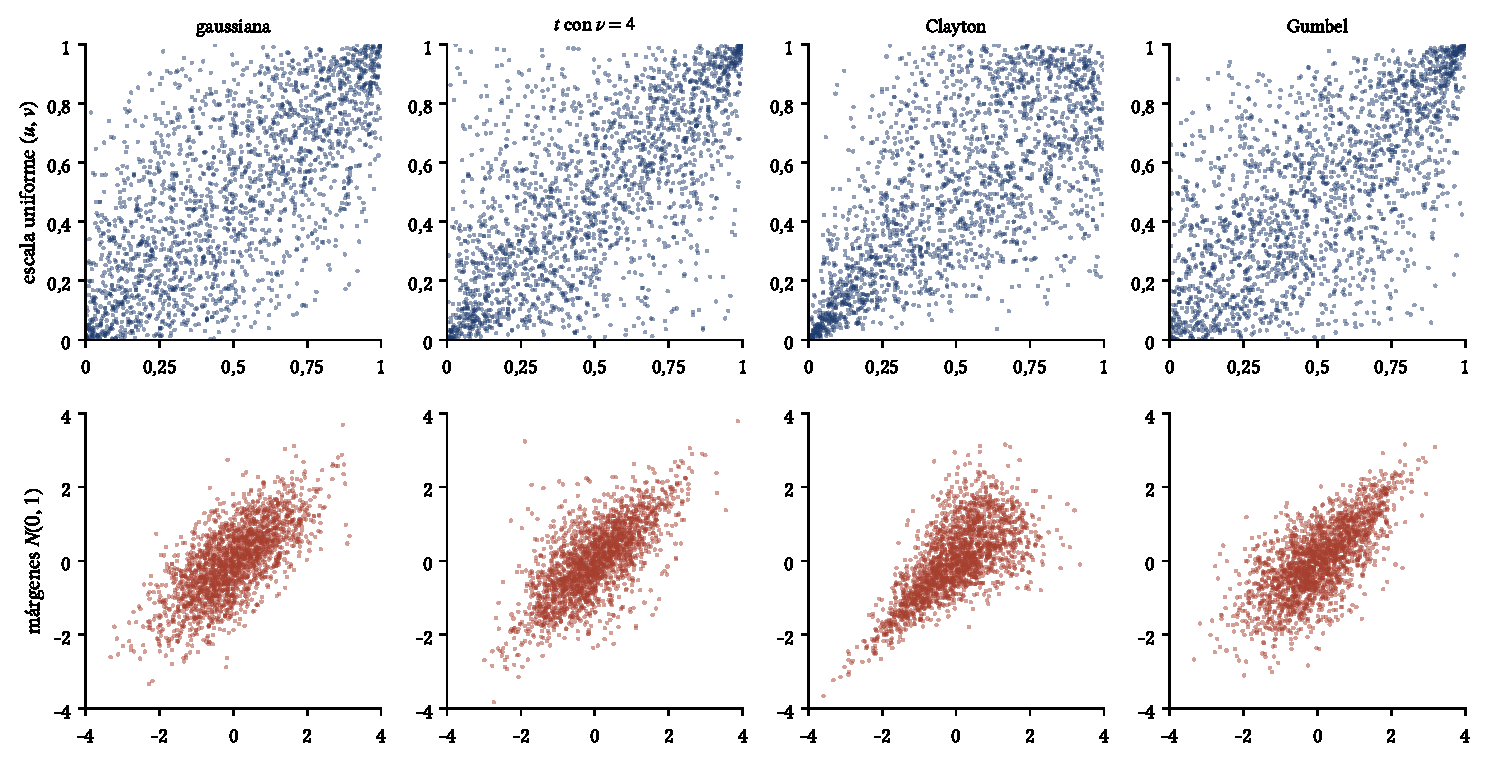
\includegraphics[width=\linewidth]{graficos/cap18_fig_copulas.pdf}
\caption{2\,000 simulaciones de cuatro cópulas con $\tau=0{,}5$ ($\rho=0{,}707$ en la gaussiana y la $t$; $\theta=2$ en Clayton y
Gumbel). Arriba, en escala uniforme; abajo, con márgenes normales, donde las diferencias en las colas se ven mejor.}
\label{fig:copulas}
\end{figure}

% ---------------------------------------------------------------------
\section{Estimación y simulación}
% ---------------------------------------------------------------------

\paragraph{Máxima verosimilitud canónica.} Como la log-verosimilitud se separa, la cópula puede estimarse sin especificar
las márgenes, sustituyéndolas por las distribuciones empíricas. Se calculan las \emph{pseudo-observaciones}
\[
  \hat u_t=\frac{\operatorname{rango}(x_t)}{n+1},\qquad \hat v_t=\frac{\operatorname{rango}(y_t)}{n+1},
\]
y se maximiza $\sum_t\ln c(\hat u_t,\hat v_t;\boldsymbol\theta)$ (Genest, Ghoudi y Rivest, 1995). Se divide entre $n+1$ y no
entre $n$ para que ningún valor sea exactamente 1, donde $\Phi^{-1}$ o $\ln(1-u)$ divergen. Si las márgenes se estiman por
separado con un modelo paramétrico y luego se estima la cópula, el método se llama de \emph{inferencia por márgenes}
(IFM; Joe, 1997). Una alternativa más simple es el \emph{método de momentos}: invertir el tau de Kendall muestral con las
fórmulas de la Proposición~\ref{prop:taukendall}.

\begin{observacion}
Las cópulas describen la dependencia de variables i.i.d. Los rendimientos diarios no lo son: su volatilidad cambia. Lo
correcto es filtrar cada serie con un modelo de volatilidad (GARCH, EWMA) y estimar la cópula de los residuos
estandarizados (el enfoque \emph{cópula-GARCH}; Patton, 2006). El Ejercicio~\ref{ej:copres} compara ambos enfoques.
\end{observacion}

\paragraph{Simulación por el método condicional.} Para simular $(U,V)$ de una cópula, se simula $U$ uniforme y luego $V$ de
la distribución condicional $C(v\mid u)=\partial C(u,v)/\partial u$, invirtiéndola en otra uniforme $W$.

\begin{proposicion}[Simulación de la cópula de Clayton]\label{prop:simclayton}
Si $U,W$ son uniformes independientes, $V=\bigl[(W^{-\theta/(1+\theta)}-1)U^{-\theta}+1\bigr]^{-1/\theta}$ tiene, junto con $U$, la
cópula de Clayton.
\end{proposicion}

\begin{proof}
La distribución condicional es la derivada parcial respecto de $u$:
\begin{align*}
  C(v\mid u) &= \frac{\partial}{\partial u}(u^{-\theta}+v^{-\theta}-1)^{-1/\theta}\\
             &= -\frac1\theta(u^{-\theta}+v^{-\theta}-1)^{-1/\theta-1}\cdot(-\theta u^{-\theta-1})\\
             &= u^{-\theta-1}(u^{-\theta}+v^{-\theta}-1)^{-(1+\theta)/\theta}.
\end{align*}
Igualamos a $w$ y despejamos $v$:
\begin{align*}
  (u^{-\theta}+v^{-\theta}-1)^{-(1+\theta)/\theta} &= w\,u^{\theta+1}\\
  u^{-\theta}+v^{-\theta}-1 &= w^{-\theta/(1+\theta)}u^{-\theta}\\
  v^{-\theta} &= (w^{-\theta/(1+\theta)}-1)u^{-\theta}+1\\
  v &= \bigl[(w^{-\theta/(1+\theta)}-1)u^{-\theta}+1\bigr]^{-1/\theta}.
\end{align*}
Como $W=C(V\mid U)$ es uniforme e independiente de $U$, el par simulado tiene la distribución condicional correcta.
\end{proof}

Para la gaussiana se simulan normales correlacionadas y se aplica $\Phi$; para la $t$, además, se divide entre
$\sqrt{W/\nu}$ con $W\sim\chi^2_\nu$ y se aplica $t_\nu$. Para Gumbel se usa el algoritmo de Marshall y Olkin (1988):
$U_i=\exp\{-(E_i/S)^{1/\theta}\}$, con $E_i$ exponenciales y $S$ una variable estable positiva de índice $1/\theta$.

% ---------------------------------------------------------------------
\section{Ejercicios resueltos}
% ---------------------------------------------------------------------

\begin{ejresuelto}{Medidas de dependencia del S\&P 500 y el Nasdaq}\label{ej:medidas}
\enunciado Describa los dos índices, calcule las correlaciones de Pearson, Kendall y Spearman, y estime la dependencia en las
colas con $\hat\lambda_L(q)=\#\{\hat u_t\le q,\hat v_t\le q\}/(nq)$ y su análogo superior para $q=10$, 5 y 1\,\%. Compare con lo
que implicaría una cópula gaussiana con el mismo tau.

\solucion
\paso{Paso 1. Márgenes.} Ambos índices tienen colas muy pesadas: curtosis 11,17 (S\&P 500) y 8,43 (Nasdaq), con volatilidades
diarias de 1,20 y 1,59\,\%.

\paso{Paso 2. Correlaciones.} Pearson $=0{,}8872$, Kendall $=0{,}7348$ y Spearman $=0{,}8919$. Si la cópula fuera gaussiana, el tau
implicaría
\begin{align*}
  \rho &= \sin\Bigl(\frac{\pi\times0{,}7348}{2}\Bigr)\\
       &= \sin(1{,}1542)\\
       &= 0{,}9145,
\end{align*}
mayor que la correlación de Pearson de los rendimientos: las colas pesadas de las márgenes reducen la correlación lineal.

\paso{Paso 3. Colas.}
\begin{center}\small
\begin{tabular}{@{}rrrr@{}}
\toprule
$q$ & $\hat\lambda_L(q)$ & $\hat\lambda_U(q)$ & Gaussiana con $\rho=0{,}9145$ \\
\midrule
10\,\% & 0,742 & 0,720 & 0,712 \\
5\,\% & 0,620 & 0,700 & 0,664 \\
1\,\% & 0,457 & 0,596 & 0,574 \\
\bottomrule
\end{tabular}
\end{center}
Con $q=1$\,\%, si el S\&P 500 está entre sus 50 peores días, el Nasdaq también lo está en el 45,7\,\% de los casos. La
gaussiana predice que esa probabilidad cae hacia cero cuando $q\to0$, pero lo hace lentamente con $\rho=0{,}91$. Los cinco peores
días del S\&P 500 fueron en septiembre a diciembre de 2008, y en los tres primeros el Nasdaq tuvo uno de sus cuatro peores días
(Figura~\ref{fig:dispersion}).

\codigoweb{cap18_ej01}
\salidaR{cap18_ej01_R.txt}
\lectura{cap18_ej01}

\RvsPy El tau de Kendall se calcula con \texttt{cor(..., method = "kendall")} en R y con \texttt{scipy.stats.kendalltau} en
Python; ambos dan la versión $\tau_b$, corregida por empates. Los rangos promedio de \texttt{rank} y \texttt{rankdata}
coinciden. La probabilidad de la normal bivariada en la diagonal, $\Phi_2(a,a;\rho)=\int_{-\infty}^a\phi(x)\Phi\bigl((a-\rho
x)/\sqrt{1-\rho^2}\bigr)dx$, se integra con la regla de Simpson en ambos lenguajes para no depender de paquetes externos
(\texttt{mvtnorm} en R).

\begin{figure}[ht]
\centering
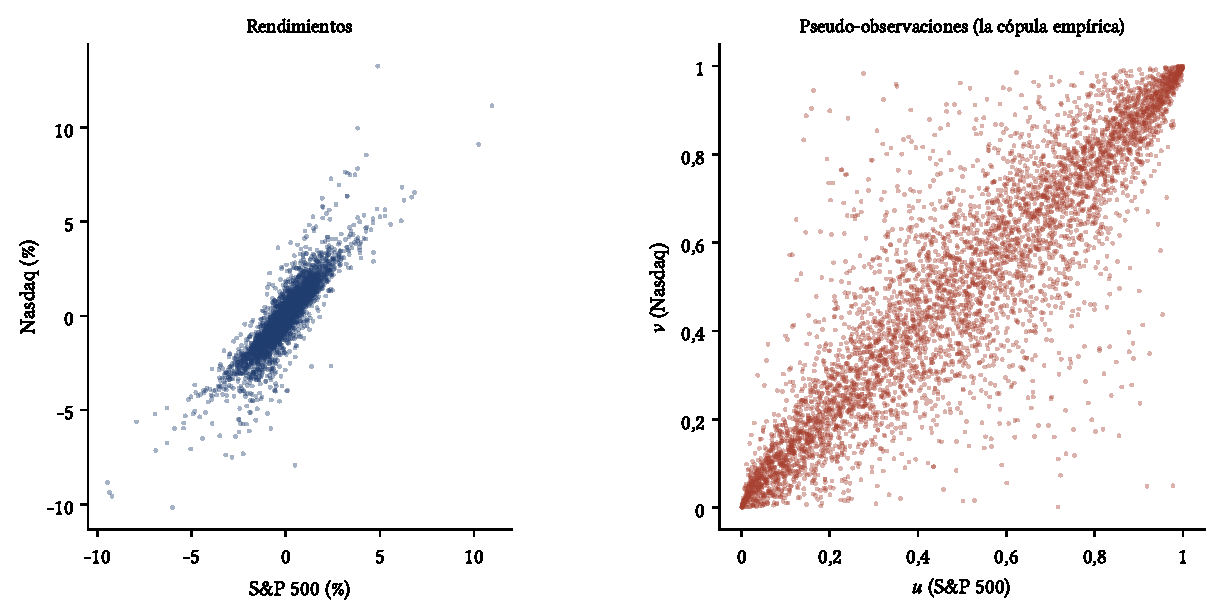
\includegraphics[width=\linewidth]{graficos/cap18_ej01_dispersion.pdf}
\caption{Izquierda: rendimientos diarios del S\&P 500 y el Nasdaq. Derecha: sus pseudo-observaciones, que eliminan el efecto de
las márgenes y muestran solo la cópula.}
\label{fig:dispersion}
\end{figure}

\begin{conclusion}
Los dos índices están muy correlacionados y su dependencia en las colas es alta, aunque con este nivel de correlación la
gaussiana se acerca a los valores empíricos hasta $q=1$\,\%. Para decidir qué cópula usar hay que estimarlas.
\end{conclusion}
\end{ejresuelto}

\begin{ejresuelto}{Estimación de cuatro cópulas}\label{ej:cuatro}
\enunciado Estime por máxima verosimilitud canónica las cópulas gaussiana, $t$, Clayton y Gumbel para los rendimientos.
Compare con AIC y con las medidas implícitas de dependencia.

\solucion
\paso{Paso 1. Resultados.}
\begin{center}\small
\begin{tabular}{@{}llrrrrr@{}}
\toprule
Cópula & Parámetros & $\ell$ & AIC & $\tau$ & $\lambda_L$ & $\lambda_U$ \\
\midrule
Gaussiana & $\rho=0{,}9008$ & 4\,189,57 & $-8\,377{,}14$ & 0,714 & 0 & 0 \\
$t$ & $\rho=0{,}9122$, $\nu=3{,}62$ & 4\,539,52 & $-9\,075{,}04$ & 0,731 & 0,666 & 0,666 \\
Clayton & $\theta=3{,}3756$ & 3\,447,99 & $-6\,893{,}97$ & 0,628 & 0,814 & 0 \\
Gumbel & $\theta=3{,}5190$ & 4\,258,52 & $-8\,515{,}04$ & 0,716 & 0 & 0,782 \\
\bottomrule
\end{tabular}
\end{center}
La cópula $t$ gana con claridad: mejora la log-verosimilitud de la gaussiana en 350 puntos con un solo parámetro más. Su
$\tau$ implícito, 0,731, es el más cercano al empírico (0,735).

\paso{Paso 2. Interpretación de $\nu$.} Para la gaussiana,
\begin{align*}
  \tau &= \frac2\pi\arcsin(0{,}9008)\\
       &= 0{,}6366\times1{,}1217\\
       &= 0{,}714 .
\end{align*}
Que $\hat\nu=3{,}62$ sea tan bajo indica dependencia fuerte en ambas colas. Clayton, que solo tiene cola inferior, es la peor:
estos datos tienen tanta dependencia en la cola superior como en la inferior. Gumbel, con su cola superior, queda segunda.

\paso{Paso 3. Momentos frente a verosimilitud.} Invirtiendo el tau empírico se obtiene $\theta=5{,}54$ para Clayton y $3{,}77$
para Gumbel, lejos de los estimadores de máxima verosimilitud (3,38 y 3,52). Cuando la familia está mal especificada, los dos
métodos estiman cosas distintas: el de momentos reproduce el tau; el de verosimilitud, la forma global de la densidad
(Figura~\ref{fig:contornos}).

\codigoweb{cap18_ej02}
\salidaR{cap18_ej02_R.txt}
\lectura{cap18_ej02}

\RvsPy Para que ambos lenguajes den los mismos parámetros, no usamos los optimizadores de cada uno (\texttt{optim},
\texttt{scipy.optimize}), que difieren en sus criterios de parada, sino una búsqueda de la sección áurea programada igual en
los dos. La cópula $t$ se estima por perfil: para cada $\nu$ de 2 a 30 se maximiza en $\rho$, y luego se refina $\nu$ con otra
búsqueda áurea. Las densidades de Clayton y de Gumbel se verificaron contra la segunda derivada numérica de $C$, y la de la $t$
contra \texttt{scipy.stats.multivariate\_t}. Los paquetes \texttt{copula} (R) y \texttt{copulae} (Python) hacen esto
automáticamente.

\begin{figure}[ht]
\centering
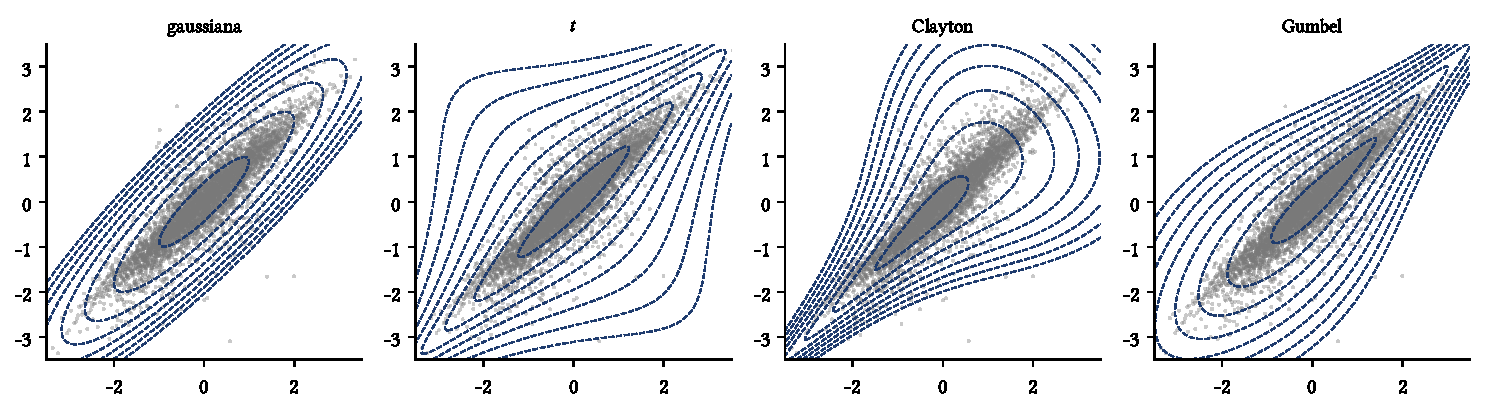
\includegraphics[width=\linewidth]{graficos/cap18_ej02_contornos.pdf}
\caption{Curvas de nivel de las cuatro cópulas estimadas con márgenes normales, sobre las pseudo-observaciones transformadas
$(\Phi^{-1}(\hat u),\Phi^{-1}(\hat v))$.}
\label{fig:contornos}
\end{figure}

\begin{conclusion}
La cópula $t$ con pocos grados de libertad es la que mejor describe la dependencia diaria entre los dos índices: alta
correlación y dependencia simétrica en ambas colas.
\end{conclusion}
\end{ejresuelto}

\begin{ejresuelto}{La cópula de los residuos estandarizados}\label{ej:copres}
\enunciado Estandarice cada rendimiento con una volatilidad EWMA ($\lambda=0{,}94$) y repita la estimación con los residuos.
Compare la dependencia en las colas antes y después de filtrar la volatilidad.

\solucion
\paso{Paso 1. Efecto del filtro.} La curtosis baja de 11,17 a 6,01 (S\&P 500) y de 8,43 a 4,55 (Nasdaq), y el tau sube de 0,735 a
0,745. La correlación de Pearson sube aún más, de 0,887 a 0,921, porque los residuos tienen colas menos pesadas.

\paso{Paso 2. Colas empíricas.}
\begin{center}\small
\begin{tabular}{@{}lrrrrrr@{}}
\toprule
 & \multicolumn{3}{c}{$\hat\lambda_L(q)$} & \multicolumn{3}{c}{$\hat\lambda_U(q)$} \\
\cmidrule(lr){2-4}\cmidrule(lr){5-7}
 & 10\,\% & 5\,\% & 1\,\% & 10\,\% & 5\,\% & 1\,\% \\
\midrule
Rendimientos & 0,742 & 0,620 & 0,457 & 0,720 & 0,700 & 0,596 \\
Residuos EWMA & 0,734 & 0,692 & 0,656 & 0,748 & 0,696 & 0,616 \\
\bottomrule
\end{tabular}
\end{center}
Con los residuos, la dependencia en la cola inferior al 1\,\% sube de 0,457 a 0,656. En los rendimientos, los días de caída más
extrema de cada índice se repartían entre episodios de alta volatilidad, en los que el otro índice también caía pero no
siempre entre sus peores días absolutos. Al dividir por la volatilidad, se comparan sorpresas relativas, que coinciden más.

\paso{Paso 3. Cópulas.} La $t$ sigue siendo la mejor, ahora con $\rho=0{,}9213$, $\nu=5{,}20$ y $\lambda=0{,}632$ (frente a
$\nu=3{,}62$ y $\lambda=0{,}666$ en los rendimientos): parte de lo que parecía dependencia en las colas era volatilidad
común. La ventaja de la $t$ sobre la gaussiana baja de 350 a 137 puntos de log-verosimilitud (Figura~\ref{fig:colas18}).

\codigoweb{cap18_ej03}
\salidaR{cap18_ej03_R.txt}
\lectura{cap18_ej03}

\RvsPy La función \texttt{ewma\_estandarizar} inicia la varianza con la media de los cuadrados de las 30 primeras observaciones;
con 5\,030 datos, el valor inicial casi no influye. Se usa el mismo filtro que en el Capítulo~\ref{cap:dcc}.

\begin{figure}[ht]
\centering
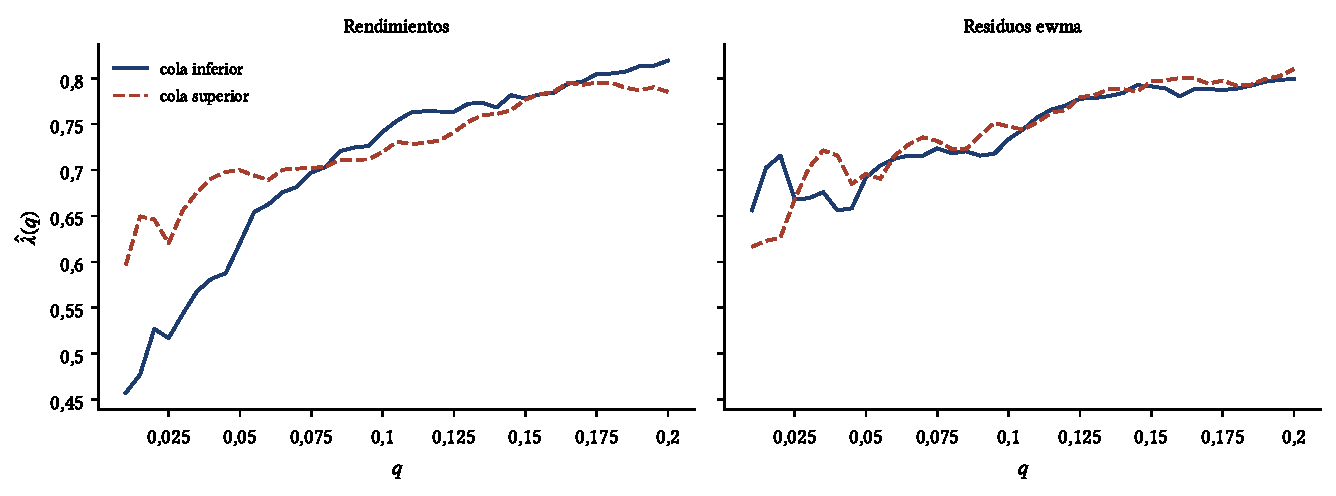
\includegraphics[width=0.9\linewidth]{graficos/cap18_ej03_colas.pdf}
\caption{Dependencia empírica en las colas $\hat\lambda(q)$ en función de $q$, para los rendimientos y para los residuos
estandarizados.}
\label{fig:colas18}
\end{figure}

\begin{conclusion}
La cópula de los rendimientos mezcla la dependencia de las sorpresas con la de las volatilidades. Filtrar primero la
volatilidad da una cópula más estable y con una interpretación más limpia, que es la que se usa para simular.
\end{conclusion}
\end{ejresuelto}

\begin{ejresuelto}{Riesgo de una cartera con cópulas}\label{ej:cartera18}
\enunciado Para una cartera con 50\,\% en cada índice, simule 20\,000 escenarios del día siguiente al 31 de diciembre de 2018
con cada cópula de los residuos, márgenes empíricas de los residuos y la volatilidad EWMA pronosticada. Calcule el VaR y el ES
al 99\,\% y compare con la independencia, la comonotonía y la simulación histórica filtrada.

\solucion
\paso{Paso 1. Escenarios.} Cada escenario es $L=-(0{,}5\,\hat\sigma_x\hat F_x^{-1}(U)+0{,}5\,\hat\sigma_y\hat F_y^{-1}(V))$, con
$(U,V)$ de la cópula, $\hat F^{-1}$ el cuantil empírico de los residuos y $\hat\sigma_x=1{,}764$\,\%, $\hat\sigma_y=2{,}102$\,\%.

\paso{Paso 2. Resultados} (pérdidas en \%).
\begin{center}\small
\begin{tabular}{@{}lrrrr@{}}
\toprule
Cópula & $\tau$ simulado & VaR 99\,\% & ES 99\,\% & VaR 99,9\,\% \\
\midrule
Gaussiana & 0,753 & 5,13 & 6,63 & 8,87 \\
$t$ & 0,760 & 5,17 & 6,66 & 8,88 \\
Clayton & 0,668 & 5,23 & 6,77 & 9,22 \\
Gumbel & 0,717 & 5,01 & 6,35 & 8,29 \\
Independencia & 0,021 & 3,68 & 4,63 & 5,76 \\
Comonotonía & 1,000 & 5,27 & 6,81 & 9,66 \\
Histórica filtrada & -- & 5,29 & 6,96 & 9,96 \\
\bottomrule
\end{tabular}
\end{center}
Con dependencia tan alta, las cuatro cópulas dan VaR al 99\,\% entre 5,0 y 5,2\,\%, cerca del de la comonotonía. Suponer
independencia subestimaría el VaR en casi un tercio:
\begin{align*}
  1-\frac{3{,}68}{5{,}17} &= 1-0{,}712\\
                         &= 0{,}288 .
\end{align*}
Clayton, con más dependencia en la cola inferior (la de las pérdidas), da el VaR al 99,9\,\% más alto; Gumbel, cuya
dependencia está en las ganancias, el más bajo.

\paso{Paso 3. La cota comonótona.} Como el ES es subaditivo, el ES de la cartera no puede superar el promedio ponderado de los ES
de cada índice, que es el ES comonótono. Con los 5\,030 residuos observados, esa cota es 7,10\,\% y el ES histórico, 6,96\,\%: la
diversificación ahorra apenas 0,13 puntos. El ES comonótono simulado (6,81) queda por debajo del histórico por el error de
simulación en la cola extrema: con 20\,000 escenarios, el ES al 99\,\% promedia solo 200 de ellos (Figura~\ref{fig:cartera18}).

\codigoweb{cap18_ej04}
\salidaR{cap18_ej04_R.txt}
\lectura{cap18_ej04}

\RvsPy Las uniformes salen del generador de Park y Miller del Capítulo~\ref{cap:eventos}, y las normales, las $\chi^2$ y las $t$
se obtienen por inversión (\texttt{qnorm}, \texttt{qchisq}, \texttt{pt} y sus equivalentes de \texttt{scipy.stats}), de modo
que R y Python simulan los mismos escenarios. Los cuantiles empíricos usan la interpolación por omisión de \texttt{quantile} y
\texttt{np.quantile}, que es la misma (tipo 7).

\begin{figure}[ht]
\centering
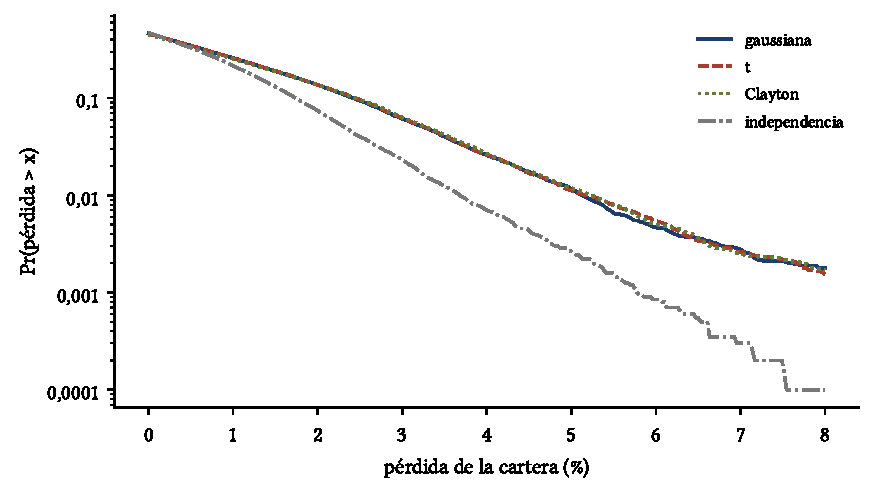
\includegraphics[width=0.78\linewidth]{graficos/cap18_ej04_colas_cartera.pdf}
\caption{Probabilidad de que la pérdida diaria de la cartera supere $x$, en escala logarítmica, según la cópula usada en la
simulación.}
\label{fig:cartera18}
\end{figure}

\begin{conclusion}
La elección de la cópula importa poco cuando los activos están casi perfectamente correlacionados, y mucho cuando se comparan
supuestos extremos como la independencia. En carteras de activos menos correlacionados (acciones y bonos, distintos países),
la diferencia entre la gaussiana y la $t$ en el VaR al 99,9\,\% es mucho mayor.
\end{conclusion}
\end{ejresuelto}

\begin{ejresuelto}{Dependencia en las crisis}\label{ej:crisis18}
\enunciado Separe la crisis financiera (julio de 2007 a junio de 2009) del resto de la muestra y estime las cópulas de los
residuos en cada parte. Calcule además el tau de Kendall en ventanas móviles de 250 días.

\solucion
\paso{Paso 1. Medidas empíricas.}
\begin{center}\small
\begin{tabular}{@{}lrrrrr@{}}
\toprule
Muestra & Días & Pearson & $\tau$ & $\hat\lambda_L$ (5\,\%) & $\hat\lambda_U$ (5\,\%) \\
\midrule
Crisis & 504 & 0,953 & 0,799 & 0,833 & 0,794 \\
Resto & 4\,526 & 0,917 & 0,740 & 0,685 & 0,681 \\
\bottomrule
\end{tabular}
\end{center}
En la crisis, la dependencia sube en todas las medidas, y más en la cola inferior.

\paso{Paso 2. Cópulas.} En la crisis, la $t$ estima $\rho=0{,}950$ y $\nu=4{,}33$, con $\lambda=0{,}727$; en el resto, $\rho=0{,}918$,
$\nu=5{,}37$ y $\lambda=0{,}619$. En ambas submuestras la $t$ tiene la mayor verosimilitud.

\paso{Paso 3. Evolución.} El tau móvil va de 0,585 (ventana que termina en agosto de 2000, en plena burbuja tecnológica) a 0,832 (ventana que termina en septiembre de 2009), con mediana 0,751
(Figura~\ref{fig:taumovil}).

\codigoweb{cap18_ej05}
\salidaR{cap18_ej05_R.txt}
\lectura{cap18_ej05}

\RvsPy Las pseudo-observaciones se recalculan dentro de cada submuestra, para que sean uniformes en ella. El tau móvil usa 228
ventanas; en R, \texttt{sapply} sobre los índices de inicio, y en Python, una comprensión de listas.

\begin{figure}[ht]
\centering
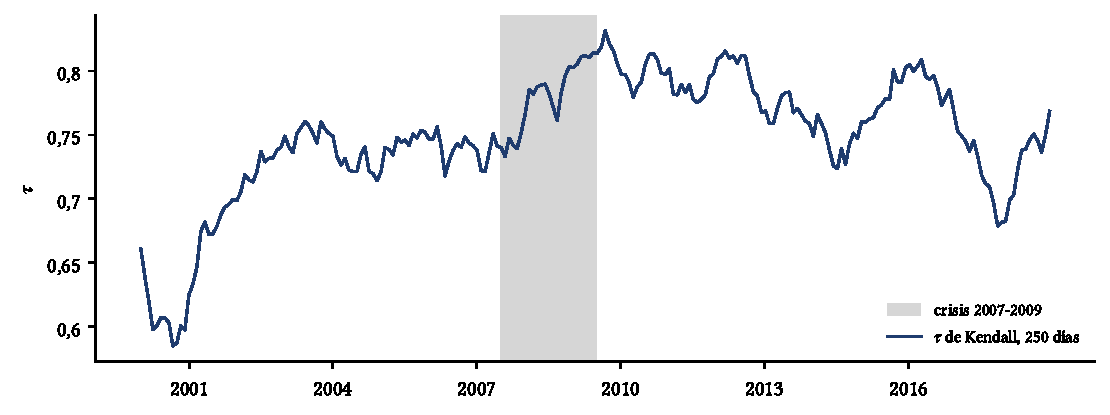
\includegraphics[width=\linewidth]{graficos/cap18_ej05_tau_movil.pdf}
\caption{Tau de Kendall de los residuos en ventanas de 250 días, fechado al final de cada ventana. En gris, la crisis de 2007--2009.}
\label{fig:taumovil}
\end{figure}

\begin{conclusion}
La dependencia no es constante: aumenta en las crisis, justo cuando la diversificación más se necesita. Una cópula estimada
con toda la muestra subestima el riesgo conjunto en esos períodos; las cópulas dinámicas (Patton, 2006) y los modelos DCC del
Capítulo~\ref{cap:dcc} abordan este problema.
\end{conclusion}
\end{ejresuelto}

% ---------------------------------------------------------------------
\section{Ejercicios propuestos}
% ---------------------------------------------------------------------

\begin{enumerate}[label=\textbf{\thechapter.\arabic*},leftmargin=*,itemsep=6pt]
  \item Para $\tau=0{,}4$, calcule el parámetro de las cópulas gaussiana, Clayton y Gumbel, y la dependencia en las colas de
  las dos últimas. \textit{Respuesta: $\rho=0{,}5878$; $\theta=1{,}333$ y $1{,}667$; $\lambda_L=0{,}5946$ y $\lambda_U=0{,}4843$.}

  \item Calcule la dependencia en las colas de una cópula $t$ con $\rho=0{,}5$ y $\nu=4$. \textit{Respuesta: $2\,t_5(-1{,}291)=0{,}2532$.}

  \item Si $X\sim N(0,1)$ e $Y=e^X$, demuestre que $\operatorname{Corr}(X,Y)=1/\sqrt{e-1}=0{,}763$, aunque la cópula es la comonotónica y
  $\tau=1$.

  \item Demuestre que la cópula de $(X,-Y)$ es $C^*(u,v)=u-C(u,1-v)$ y que su tau de Kendall es $-\tau$.

  \item Demuestre que la cópula de Clayton tiende a la de independencia cuando $\theta\to0$ y a la comonotónica cuando
  $\theta\to\infty$.

  \item \emph{(Simulación.)} Simule 500 muestras de $n=1\,000$ de una cópula $t$ con $\rho=0{,}7$ y $\nu=4$, y estime en cada una la
  gaussiana y la $t$. ¿En qué porcentaje de muestras gana la $t$ por AIC? ¿Cuál es el sesgo de $\hat\nu$?

  \item \emph{(Con datos de la BVL.)} Estime la cópula entre los rendimientos diarios del índice S\&P/BVL Perú General y del
  precio del cobre. ¿Hay más dependencia en las caídas que en las subidas?

  \item \emph{(Con datos.)} Con los precios de Apple y Alphabet del Capítulo~\ref{cap:eventos}, repita los
  Ejercicios~\ref{ej:cuatro} y \ref{ej:copres}. ¿Es la dependencia entre dos acciones del mismo sector parecida a la de dos índices?
\end{enumerate}

% ---------------------------------------------------------------------
\section{Resumen de fórmulas}
% ---------------------------------------------------------------------

\begin{table}[H]
\centering\small
\begin{tabular}{@{}ll@{}}
\toprule
Concepto & Fórmula \\
\midrule
Sklar & $H(x,y)=C(F(x),G(y))$;\quad $h=c(F,G)\,f\,g$ \\
Fréchet-Hoeffding & $\max(u+v-1,0)\le C(u,v)\le\min(u,v)$ \\
Gaussiana & $c=\frac{1}{\sqrt{1-\rho^2}}\exp\bigl(-\frac{\rho^2(x^2+y^2)-2\rho xy}{2(1-\rho^2)}\bigr)$;\quad $\tau=\frac2\pi\arcsin\rho$;\quad $\lambda=0$ \\
$t$ & $\tau=\frac2\pi\arcsin\rho$;\quad $\lambda_L=\lambda_U=2t_{\nu+1}\bigl(-\sqrt{(\nu+1)(1-\rho)/(1+\rho)}\bigr)$ \\
Clayton & $C=(u^{-\theta}+v^{-\theta}-1)^{-1/\theta}$;\quad $\tau=\frac{\theta}{\theta+2}$;\quad $\lambda_L=2^{-1/\theta}$ \\
Gumbel & $C=\exp\{-[(-\ln u)^\theta+(-\ln v)^\theta]^{1/\theta}\}$;\quad $\tau=1-\frac1\theta$;\quad $\lambda_U=2-2^{1/\theta}$ \\
Pseudo-observaciones & $\hat u_t=\operatorname{rango}(x_t)/(n+1)$ \\
Cola empírica & $\hat\lambda_L(q)=\#\{\hat u_t\le q,\hat v_t\le q\}/(nq)$ \\
\bottomrule
\end{tabular}
\caption{Fórmulas principales del Capítulo 18.}
\end{table}

\section*{Referencias}
\begin{itemize}[leftmargin=*]
  \item Demarta, S. y McNeil, A. J. (2005). The $t$ copula and related copulas. \emph{International Statistical Review}, 73(1),
        111--129.
  \item Embrechts, P., McNeil, A. J. y Straumann, D. (2002). Correlation and dependence in risk management: Properties and
        pitfalls. En M. Dempster (ed.), \emph{Risk Management: Value at Risk and Beyond}, 176--223. Cambridge University Press.
  \item Genest, C., Ghoudi, K. y Rivest, L.-P. (1995). A semiparametric estimation procedure of dependence parameters in
        multivariate families of distributions. \emph{Biometrika}, 82(3), 543--552.
  \item Genest, C. y MacKay, J. (1986). The joy of copulas: Bivariate distributions with uniform marginals. \emph{The American
        Statistician}, 40(4), 280--283.
  \item Joe, H. (1997). \emph{Multivariate Models and Dependence Concepts}. Chapman \& Hall.
  \item Lindskog, F., McNeil, A. J. y Schmock, U. (2003). Kendall's tau for elliptical distributions. En G. Bol et al. (eds.),
        \emph{Credit Risk: Measurement, Evaluation and Management}, 149--156. Physica-Verlag.
  \item MacKenzie, D. y Spears, T. (2014). `The formula that killed Wall Street': The Gaussian copula and modelling practices
        in investment banking. \emph{Social Studies of Science}, 44(3), 393--417.
  \item Marshall, A. W. y Olkin, I. (1988). Families of multivariate distributions. \emph{Journal of the American Statistical
        Association}, 83(403), 834--841.
  \item McNeil, A. J., Frey, R. y Embrechts, P. (2015). \emph{Quantitative Risk Management}, ed. revisada, cap. 7. Princeton
        University Press.
  \item Nelsen, R. B. (2006). \emph{An Introduction to Copulas}, 2.ª ed. Springer.
  \item Patton, A. J. (2006). Modelling asymmetric exchange rate dependence. \emph{International Economic Review}, 47(2),
        527--556.
\end{itemize}
